
\documentclass[11pt,a4paper]{article}

\usepackage{fouriernc}
\usepackage[utf8]{inputenc}
\usepackage[T1]{fontenc}
\usepackage[english]{babel}
\usepackage{graphicx}
\usepackage{amssymb}
\usepackage{amsmath}
\usepackage{natbib}
\usepackage{a4wide}
\usepackage[small]{caption}
\usepackage{url}
\usepackage{booktabs}
\usepackage[output-decimal-marker={,},list-final-separator={ en }]{siunitx}
\usepackage[pdfusetitle]{hyperref}
\usepackage{listings}

\linespread{1.3}
\usepackage{mathrsfs,amsmath} 
% \renewcommand{\arraystretch}{1.5}
\usepackage{tabularx}
\usepackage{rotating}
\usepackage{float}
\usepackage{pdflscape}
\usepackage[utf8]{inputenc}

\lstset{
language=C,
basicstyle=\small\sffamily,
numbers=left,
numberstyle=\tiny,
frame=tb,
columns=fullflexible,
showstringspaces=false
}

\graphicspath{{../data/figs/}} %Setting the graphicspath

\title{CP II; Membrane Simulation}
\author{Brandon Parfimczyk \& Kien Do}
\date{30-03-2020}

\begin{document}

\maketitle

\tableofcontents
\newpage

\section{Manual}

\begin{enumerate}
\item Compiling: Run 'make all' in the project root folder). This compiles all
	the tests and the main program into the "./executables/" folder.
\item for main program: change directories to ../executables and run '
	./membrane-sim' (for more information and help use -h) 
\item if all *.dat have been created, calculate observables and get graphs for
	numerical analysis: ../data/gen\_e\_violation.sh and ../data/gen\_pos\_mom 
\item generate *.png for visualizations ../data/extract\_e\_violation\_p.sh and
	../data/extract\_pos\_mom 
\item to get the animation of the membrane in *.gif go to ../data/gnuplot and
	gnuplot >> load 'arr\_3d\_gif.plt'
\end{enumerate}

\section{Planning}

The planning in this project was the following:

03.03 - Assemblance, read the notes and implement the algorithm for the integrators, discuss the skeleton of the main program\\

07.03. - restructuring of codes and generalization for potentials in integrator algorithms\\

10.03. - implement the initial conditions\\

14.03. - make the plots and animations, discuss how to obtain the continuous cases from the discretizations\\

22.03. - discuss results\\

30.03. - finalize everything in report.\\

\section{Physical Transcription}
In this project we want to determine the time evolution of a membrane in two dimensions, modeled by the Hamiltonian
\begin{equation}\label{Eq: Ham}
\hat{H} = \sum_{n_{1}, n_{2} = 0}^{N} a^{2} \left\{ \frac{1}{2} \pi^{2}(\mathbf{n}) - \frac{1}{2} h \hat{\nabla}^{2} h(\mathbf{n}) + V(h(\mathbf{n}))\right\}.  
\end{equation}
$h$ stands for the displacement of the membrane and the potential will be:
\begin{equation}
V(h(\mathbf{n})) = \frac{\lambda}{4!} h^{4}
\end{equation}
Just like in previous projects we are using a discretization of space and time ($\mu \in (0,1)$):
\begin{align}
	T & = \tau * \text{RUNS} \\
n_{\mu} & \in \frac{1}{N - 1} (0, 1, ..., N - 1).
\end{align}
For this project we don't implement Periodic Boundary conditions anymore, insted we fix our boundaries to
\begin{equation}
h(\mathbf{n}) = 0,
\end{equation}
for $\exists \mu: n_{\mu} = 0.$\\
We can derive the equations of motion with the Hamilton formalism and acquire
\begin{equation}\label{Eq: PDE1}
\ddot{h}_{t} = \hat{\nabla}^{2} h(\mathbf{n}) - V'(h(\mathbf{n}))
\end{equation}
We will solve this by using two symplectic integrators: (\textbf{a}) Leapfrog
(2nd order) and (\textbf{b}) Yoshida (4th order) integrator. The results will
be displayed and analyzed in physical and numerical terms. The project will be
concluded by finding suitable values for the quantities linear lattice size $N$
and integration timestep $\tau$ to have a meaningful appoximation to the
continuous system.


\section{Code Recycling}

We can use some code of the previous project. This includes the codes for
generating indices from coordinates and vice versa and parts of code for the
Laplacian, since this already uses the nearest neighbours. The recycled
functions are:

In Module [geometry.c]:
\begin{enumerate}
    \item $\texttt{ind2coord()}$
    \item $\texttt{coord2ind()}$
	\item $\texttt{nn\_neighbour()}$ (with modifications for the non PBC)
    \item $\texttt{nn\_create()}$
\end{enumerate}
In Module [functions.c]:
\begin{enumerate}
	\item $\texttt{laplace\_arr()}$ (with modifications for the non PBC)
\end{enumerate}

This will now ignore the points which are border points of our system. The array
is created by the function \verb|is_border_create()| which saves the information of
\verb|is_border(int index)| for all indices. We save routines in the Laplacian by doing
this.

We do not have to implement the non PBC explicitly in the integrators when the
inital conditions for all border points in the pi array are zero. The border
points will be updated but it is just adding zeroes. When the boundaries are not
equal 0 then the simulation will have a constant drift into the direction of the
momentum at the borders and will not be physical anymore. Care if changing the
boundary conditions. You will have to modify the integrators to ignore the
boundary points at all. The following code snippet could be useful for this:

\begin{figure}[H]
	\begin{lstlisting}
for (int ind = 0; ind < ipow(N, D); ind++) {
	if (is_border_arr[ind]) {
		out[ind] = h[ind];
		continue;
		}
	}
	\end{lstlisting}
\end{figure}

\section{Modules and some relevant functions}

 Module [\verb|[functions.c]|] contains 
 \begin{itemize}
	 \item \verb|is_border()| checks wether our index is a border point.
	 \item  \verb|laplace_arr()| to calculate the laplace acting on the
		 displacement in Eq. (\ref{Eq: Ham})
	 \item \verb|dpolynom()| was \verb|laplace_arr()| to calculate the laplace
		 acting on the displacement in Eq. (\ref{Eq: Ham}).firstly being
		 implemented for a generic power potential. To generalize the
		 implementation of a more generic potential, see [\verb|potentials.c|].
 \end{itemize} 

 Module [\verb|initial_cond.c|] contains
 
\begin{itemize}
	\item \verb|init_h_pyramid_a()| to set up the initial condition for our
		differential equation (\ref{Eq: PDE1}). It is an approximate pyramid. \\
		Achieved by putting identical triangles next to each other on top of the
		base, a $(N-1)x(N-1)$ square along axis 1. The object looks like the
		roof of a typical dream house of a four headed family now.\\ Then
		identify (on the base) the set of points (two triangles) where we have
		to do the same as in the previous step, but now along axis 0.
	\item \verb|init_h_pyramid_b(|) is another initial condition. However, the
		edges from the top of the pyramid don't connect to the corners of the
		base square.
	\item \verb|init_pi_zero()| sets all our initial $\pi_{0}$ to 0.
\end{itemize}

 Module [\verb|integrators.c|] contains
\begin{itemize}
	\item \verb|integ_set_integrator()| which basically points at the address of
		one of the available integrators below.
	\item \verb|leapfrog()|
	\item \verb|integ_yoshida()|
\end{itemize}

 observables.c contains
\begin{itemize}
\item $\texttt{hamilton()}$ calculates the energy of the system at the integeration time $t$ given we know the displacement $h_t$ and $\pi_t$ 
\end{itemize} 

 potential.c contains
\begin{itemize}
\item $\texttt{pot\_set\_func()}$ which basically points at the address of one of the available potentials below for the energy calculation or their respective derivative for the usage of the integrators. 
\end{itemize}

\subsection{Note: Challenge encountered in implementing a generic potential}
Different from the project qunatum mechanical particle in a potential where we had a potential which was not dependent on the state of the particle (here: displacement of the membrane at position $\mathbf{n}$) we had to think how to implement a generic potential, Brandon came up with the idea to use pointers. We implemented the potentials (the computer reserves an address for them) needed beforehand and in need we just use a function $ \texttt{pot\_set\_func()}$ which points at the adress in question. This way we didn't need to hardcode a specific potential in the algorithm of the integrator.

\section{Main program: membrane-sim.c}

By defining the preprocessor token \verb|'MAINPROGRAM'| in all the main programs
we can get the global variables defined inside main source file and extern in
all modules by \verb|global.h|.
This enables us to change global variables at runtime. We use this for the
command line handling. All the possible options are:

\begin{figure}[H]
	\begin{lstlisting}
Usage: membrane-sim [options]...

The following options are available:
    -N <integer>    number of lattice points in one dimension, positive integer
    -D <integer>    number of dimensions, positive integer
    -i <integer>    choice of integrator:
                        0    yoshida integrator
                        1    leapfrog integrator
    -p <integer>    choice of potential:
                        0    no potential
                        1    higgs potential
    -w <double>     set param0 for use in potential
    -t <float>      time step tau for a single integration step
    -T <float>      ending time t_end
    -e <integer>    output observables and field arrays only every <integer>th
                    time integration step
    -f <file>       write output field to "<file>" and observables to
                    "<file>_obs"
                    if the specified filename has an filetype extension then
                    the resulting observable file will share the same extension
                    e.g.    simulated_system.dat -> simulated_system_obs.dat
                            membrane_sys -> membrane_sys_obs
                    if this option is not specified the program will print the
                    field array data to stdout and omit printing observables
    -h              show this help text
	\end{lstlisting}
\end{figure}

In the program we can choose the initial coordinates to place the top of the pyramid and the height of the pyramid. \\
Using $\texttt{pot\_set\_func()}$ and $\texttt{integ\_set\_integrator()}$ we can choose the integrator and potential to work with. $\texttt{integ\_integrator()}$ then performs the integration until T has been reached. The program also calculates the energy and the energy difference of the system at the point of time 0 and $t$ and also the displacement and its velocity at the middle of the field and saves it in a seperate file.

\section{Testing}

\subsection{NN-Testing}

This had to be modificated to work with the non PBC in this project.

\subsection{Testing Leapfrog And Yoshida Integrator}

To test wether both integrators do their job like intended we used them on a very simple system of differential equation of a free falling object:
\begin{align}\label{Eq: ODE1}
\dot{v} &= -g \\
\dot{x} &= v.
\end{align}

So we chose N = D = 1, since we have a single object instead of a field. In the algorithm of an integrator the calculation of the acceleration is crucial for example in [integrators.c] $\texttt{leapfrog()}:$ \\
We have to set $\texttt{pot\_deriv\_func(h[n]) =  h\_F[n] + g}$. Since $N = 1$ and the boundary conditions of $\texttt{laplace\_arr()}$ ($ h_{F}[0] = h[0]$) we implement

\begin{figure}[H]
\begin{lstlisting}
double pot_deriv_newt_grav(double h)
{
return h + g_newt;
}
\end{lstlisting}
\end{figure}
The test is succesful, if the difference with the analytical solution of the ODE [\ref{Eq: ODE1}] is below machine precision:
\begin{equation}
x(t) = -\frac{g}{2} t^{2} + v_{0} t + x_{0}.
\end{equation}

\subsection{Testing Approximation Of Continous Pyramid}

The test is summing all displacement values together and compares it with the analytical volume of an exact pyramid:
\begin{equation}
V = \frac{1}{3} A_{sq} * h.
\end{equation} 
In theory we just need to do $N \rightarrow \infty$ and the difference should approach $0$. Finite ressources can't achieve this.\\
But if there is a bijective relationship of a geometrical object to a volume formula, all we have to do is see wether with scaling N, the difference is monotoneous decreasing. \\
In doubt we plotted the initial condition, as one can see if one runs the script ../data/gnuplot/arr\_3d\_init.plt.\\

\subsection{Testing Linearity Of Laplace Function}

test\_functions: $\texttt{ [laplace\_arr()} $ basically just applies first the laplace operator on two summands and adds them together and second applies laplace on the sum of both summands and comapres both. The difference is being divided by the Volume of the lattice to avoid scaling errors.


\section{Result}

\subsection{Physical analysis}

Eq. [\ref{Eq: Ham}] which decribes the energy of the system. Calculating the
time derivative analytically of this function gives 0. That means that energy
should be conserved. Looking at the observable \verb|*_obs.dat| we see that the
average error stays constant (up to a certain digit after the comma), which
hints that we did something right. Increasing the integration time step $\tau$
should decrease the energy difference even more. We agreed on that $\tau$ is
small enough if the energy difference is in order of machine precision
(\num{e-15}). \\
In the case of having no potential and choosing the initial conditions to be in
a middle of the pyramid we actually see a standing wave emerging as the mebrane
simply just moves up and down, what was to be expected. \\
In the case of using the Higgs potential the animation shows a non trivial
time evolution of the membrane. As the pyramid like
initial condition flattens (non uniformly) and the wave starts to spread out, it
doesn't recover the pyramid back as the waves hit the boundaries and come back
and interferes. One sees that there are more than just one mode occuring (one
can see it more clearly, when viewing it from the side as in some point of time
the field is partially positively displaced and partially negatively displaced.)

\subsection{Numerical analysis}

\begin{figure}[H]
\centering
	\fbox{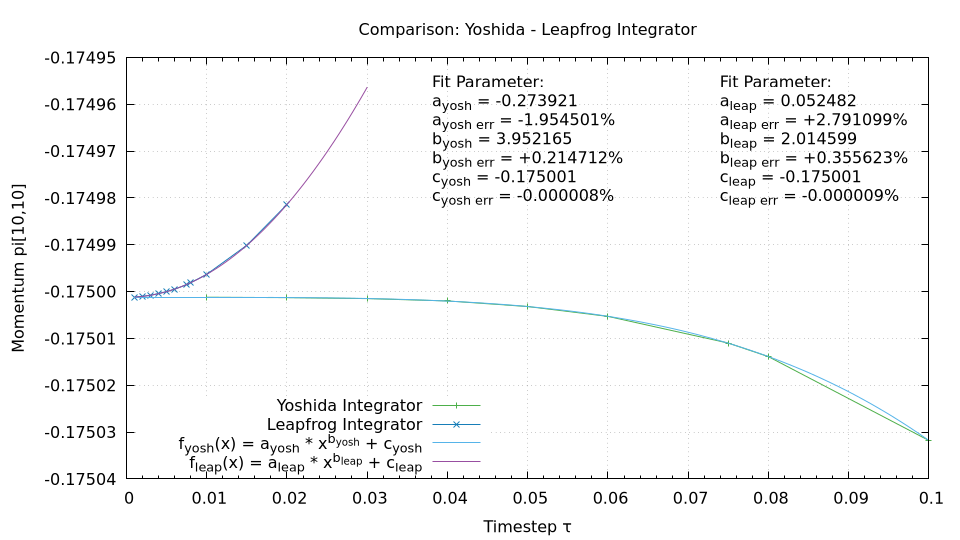
\includegraphics[width=\textwidth]{obs_mom_tau_comparison.png}}
\caption{Momentum at T = 12 versus integrator time step for both integrators.}
\label{Fig: obs_mom_tau_comp}
\end{figure}

\begin{figure}[H]
\centering
	\fbox{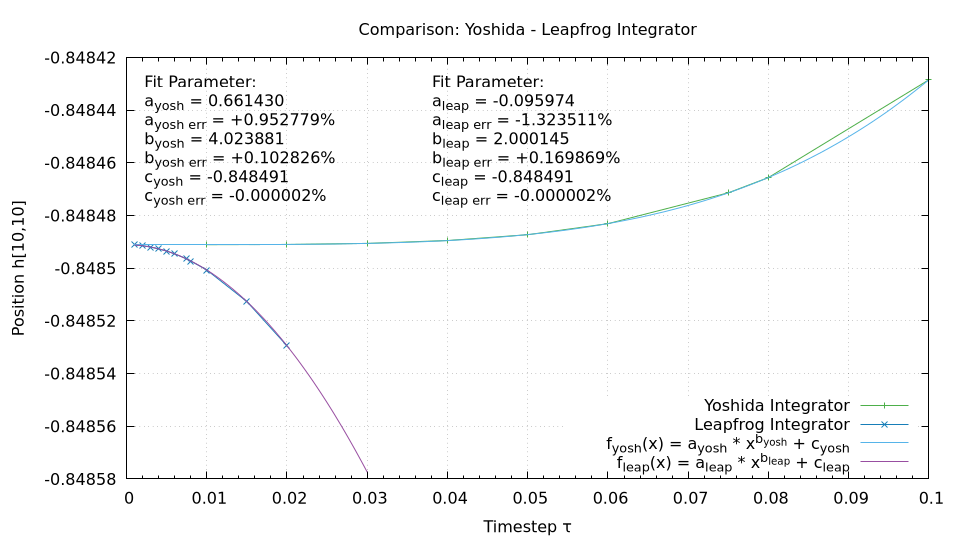
\includegraphics[width=\textwidth]{obs_pos_tau_comparison.png}}
\caption{Position at T = 12 versus integrator time step for both integrators.}
\label{Fig: obs_pos_tau_comp}
\end{figure} 


In fig. [\ref{Fig: obs_mom_tau_comp}] we can see that the fit parameter give us
the right results. (b = 2 und b = 4) we get the right orders for $\tau$ for the
respective integrators back. It also tells us that if we want to calculate an
observable with one magnitude higher precision, we need to choose $\tau
\rightarrow \tau \cdot 10^{-\frac{1}{\text{order of integrator }}} $. From this
figure we can not read off a good value for $\tau$. However, we see the
behaviour that both integrators approach the value $-0.175$ for the momentum as
$\tau$ goes to 0. A similar observation can be made in fig.  [\ref{Fig:
obs_pos_tau_comp}]

\begin{figure}[H]
\centering
	\fbox{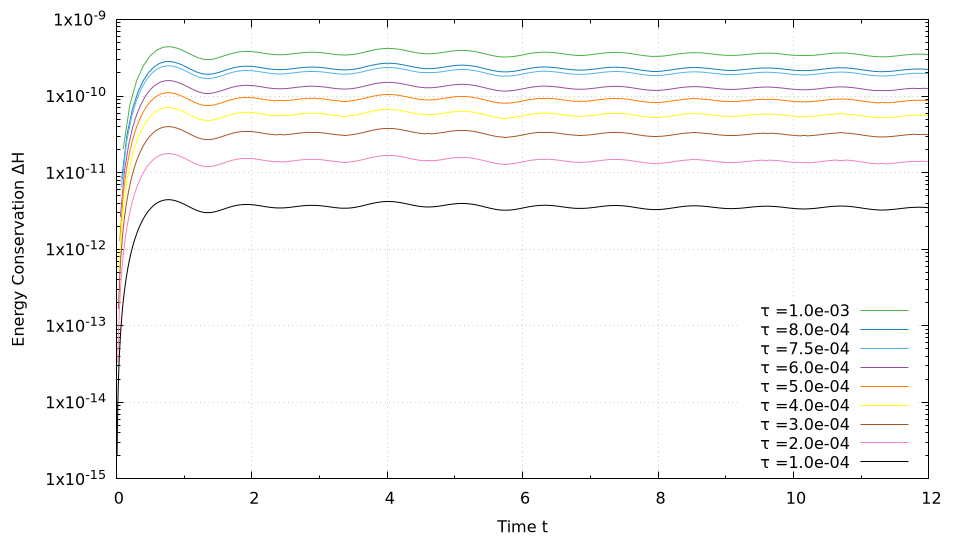
\includegraphics[width=\textwidth]{all_obs_e_vio_leap.png}}
\caption{energy difference from t=0 and at time t versus the time with the leapfrog integrator}
\label{Fig: all_obs_e_vio_leap}
\end{figure}

\begin{figure}[H]
\centering
	\fbox{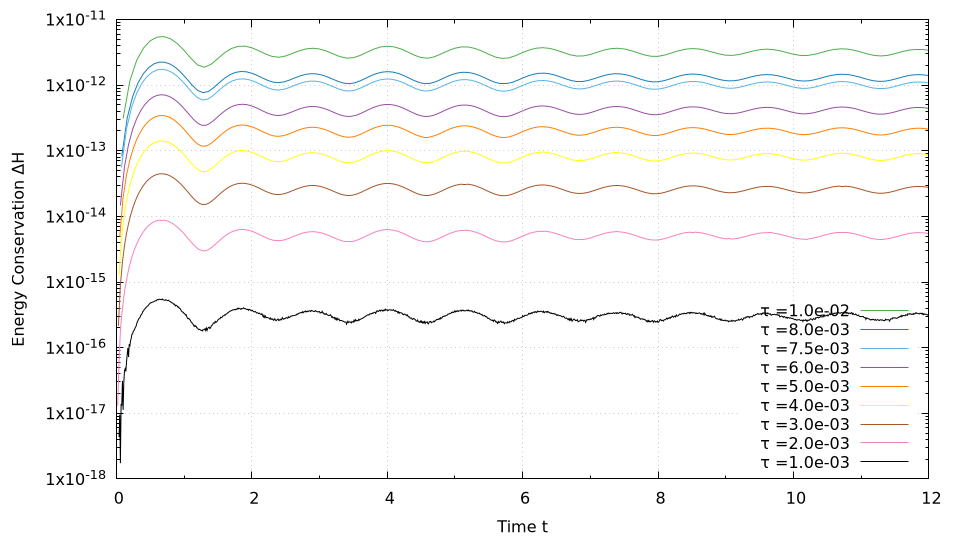
\includegraphics[width=\textwidth]{all_obs_e_vio_yosh.png}}
\caption{energy difference from t=0 and at time t versus the time with the yoshida integrator}
\label{Fig: all_obs_e_vio_yosh}
\end{figure}

In fig. [\ref{Fig: all_obs_e_vio_leap}] and [\ref{Fig: all_obs_e_vio_yosh}] we
calculated the energy difference of the field at time 0 and time t for a field
with linear size $N = 21$ and several values for $\tau$. We see that the yoshida
integrator needs only a value of $\tau = 1e-3$ such that we get a good
approximation. The Leapfrog integrators needs a $\tau$
magnitudes lower than that to achieve this.

\begin{sidewaysfigure}
\centering
	\fbox{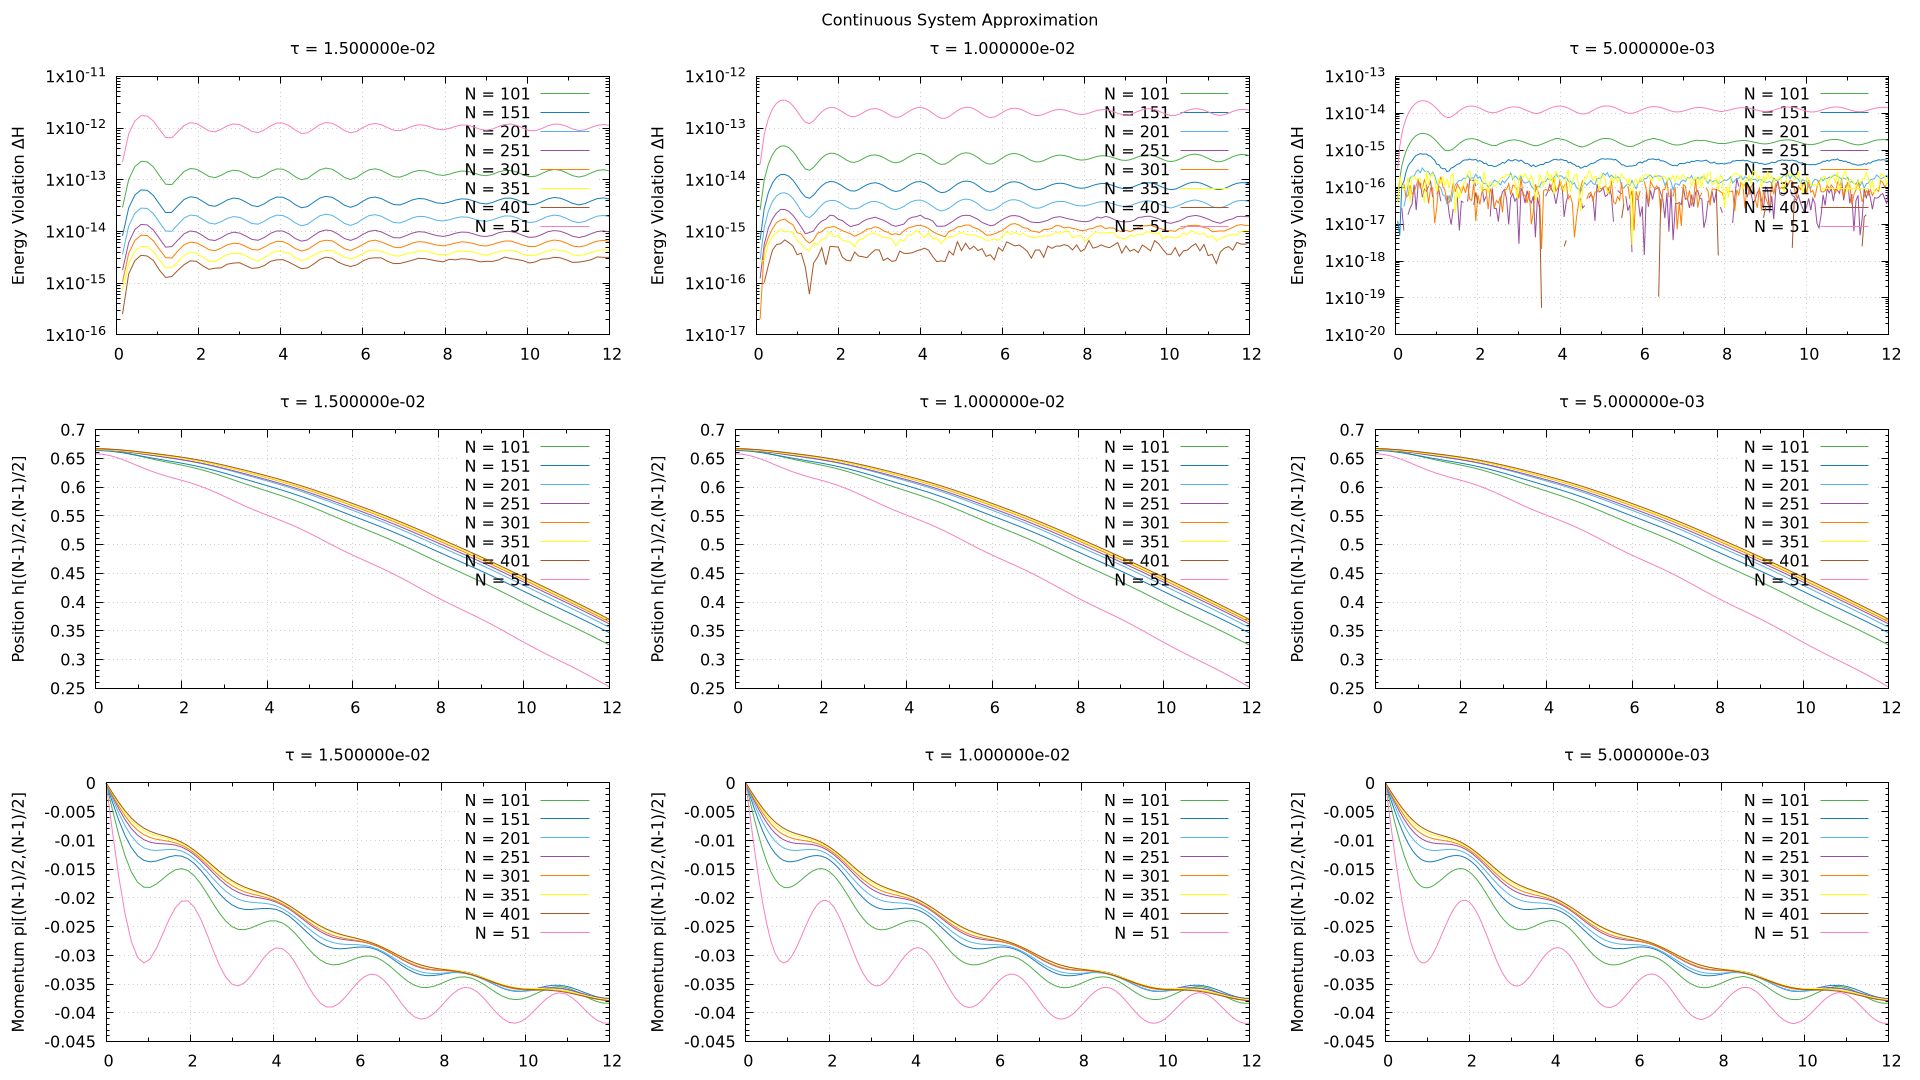
\includegraphics[width=\textwidth]{obs_cont_sys_e.png}}
\caption{for different values of tau each graph shows the observables for multiple N's with yoshida integrator}
\label{Fig: obs_cont_sys_e}
\end{sidewaysfigure}

\begin{sidewaysfigure}
\centering
	\fbox{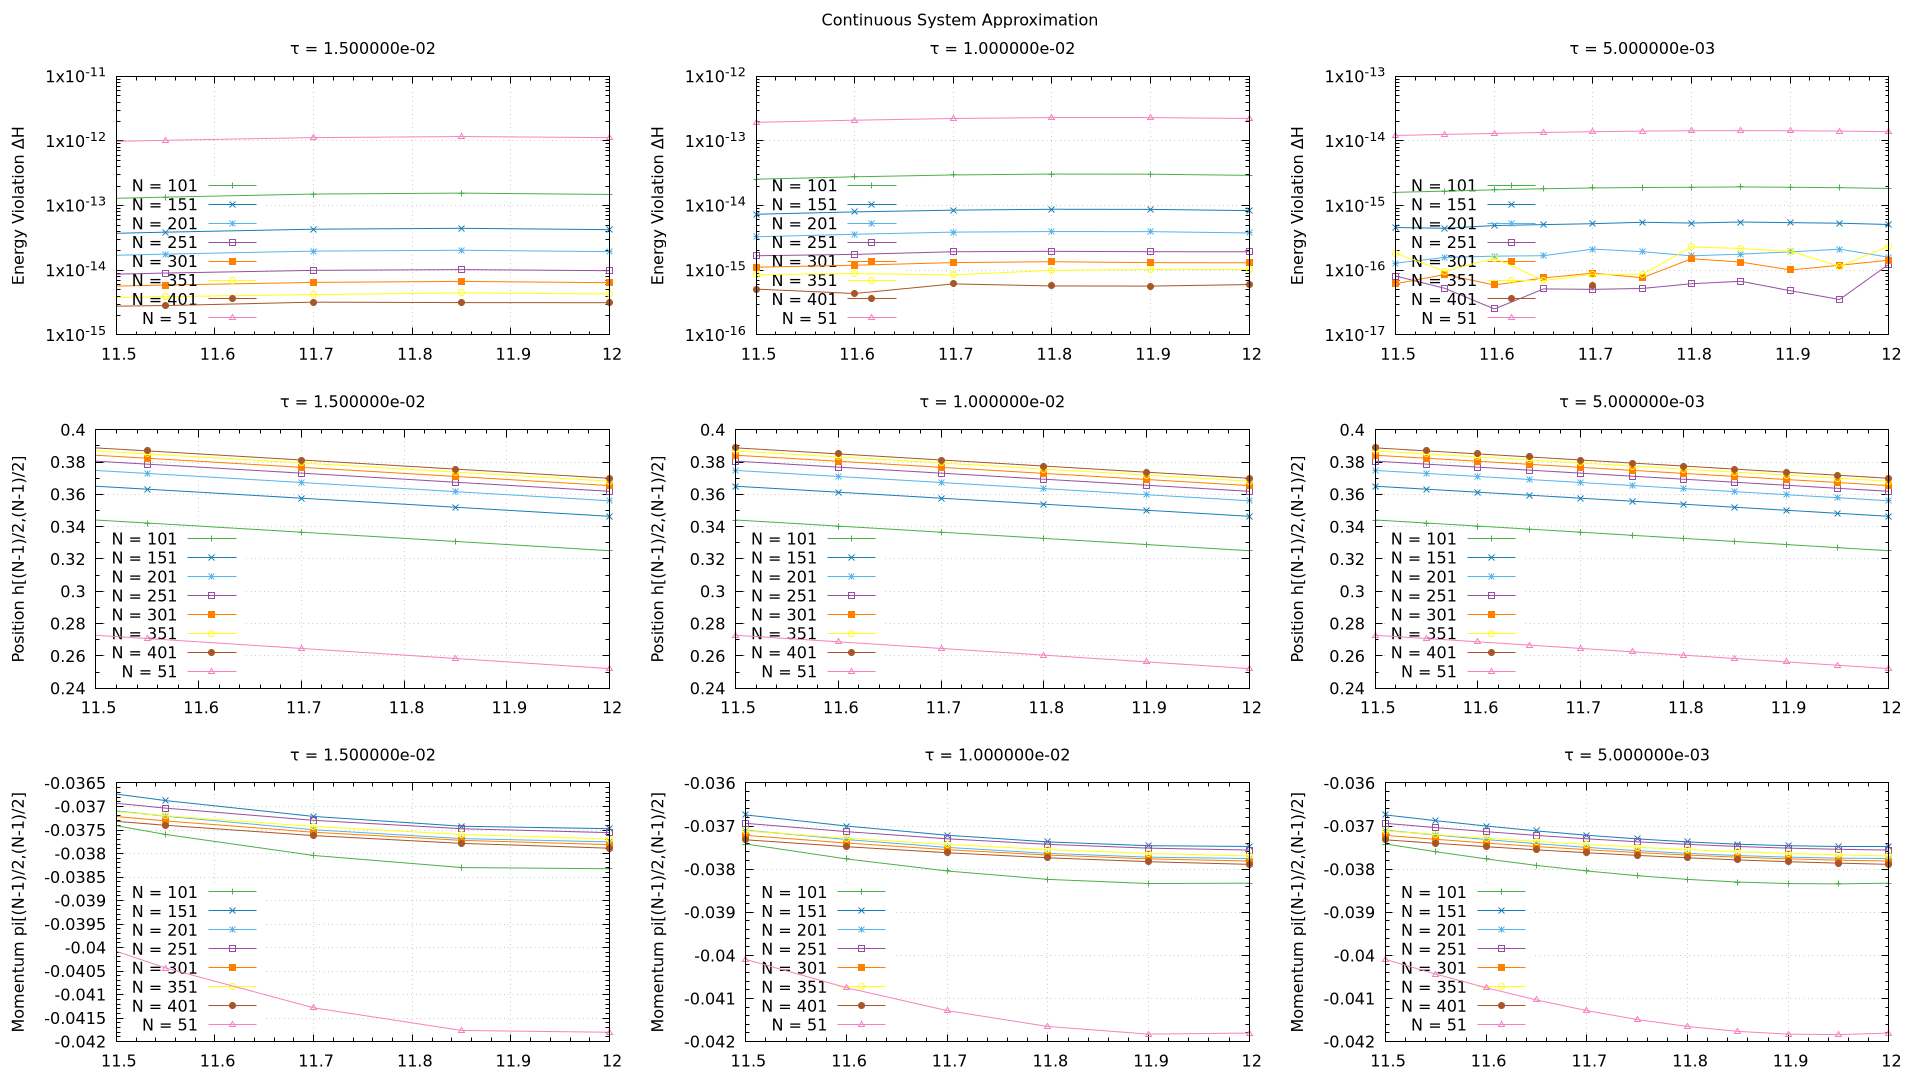
\includegraphics[width=\textwidth]{obs_cont_sys_e_zoom.png}}
\caption{for different values of tau each graph shows the observables for multiple N's with yoshida integrator - zoomed in}
\label{Fig: obs_cont_sys_e_zoom}
\end{sidewaysfigure}

In fig. [\ref{Fig: obs_cont_sys_e}] we tried to find out how to choose $N$ and
$\tau$ such that we obtain a good approximation to the continuous case. It turns
out that the higher $N$ is the smaller the energy difference. Such that for a
given $N$ once we found a suitable $\tau$, we can choose any smaller $\tau$ and
we would still recover the continuous case. Vice versa with given $\tau$ and the
choice for $N$, as with increasing $N$ the observable values start to converge
to certain values. This can be seen in fig. [\ref{Fig: obs_cont_sys_e_zoom}]
more clearly.\\

We decided on $N = 401$ and $\tau = \num{5.0e-03}$. The Question is to which
decimal place do you want to have the observables precise. In fig [\ref{Fig:
initial_condition}] you can see the initial condition for those values. Inside
the \verb|./data/figs/| folder is a animation \verb|anim.gif| for this case.
There are also the plots of the observables for the $N = 21$ case for different
values of $\tau$. They are all so close that you can not differentiate them
without zooming.

\begin{figure}[H]
\centering
	\fbox{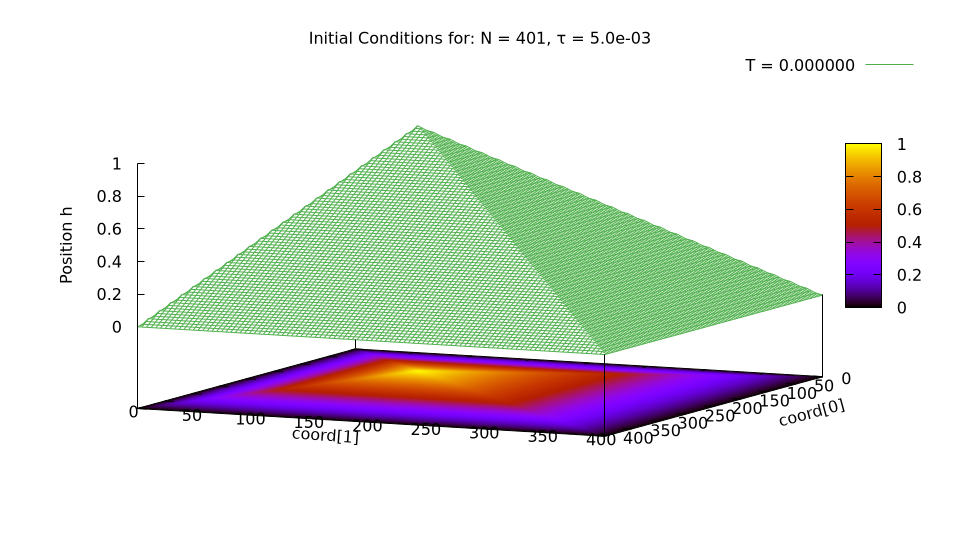
\includegraphics[width=\textwidth]{init_condition.png}}
\caption{Initial condition of the field. We pull the membrane and this gives approximatively a pyramid}
\label{Fig: initial_condition}
\end{figure}

\section{Extension to more than two dimensions}

Except of the animation one might try to find similar analysis for higher
dimensions. The whole program is written with a variable dimension. Only the
test for the \verb|is_border()| function and the pyramid starting condition are
only working for 2-D.


\end{document}


